
\documentclass[a4paper,12pt]{article}
\usepackage{vntex}
\usepackage{a4wide, fancyhdr}
\usepackage{amsmath}
\newcommand\numberthis{\addtocounter{equation}{1}\tag{\theequation}}
\usepackage{amsthm}
\usepackage{float}
\usepackage{multicol,longtable,amscd}
\usepackage[framemethod=tikz]{mdframed}% For highlighting paragraph backgrounds
\usepackage{caption,subcaption}
\usepackage{tabularx} % in the preamble
\usepackage{tikz}
\usetikzlibrary{shapes, calc, shapes, arrows}
\usepackage{pgfplots}
\usepackage{bbm}
\usepackage{titletoc,tocloft}
\DeclareMathOperator*{\argminB}{argmin} 
\DeclareMathOperator*{\argmaxB}{argmax} 
\setlength\arrayrulewidth{0.2pt}
\usepackage{textcomp}
\usepackage{xcolor}
\usepackage{color}

\usepackage{lastpage}
\usepackage[lined,boxed,commentsnumbered]{algorithm2e}
\usepackage{enumerate}
\usepackage{graphicx}							% Standard graphics package
\usepackage{array}
\usepackage{tabularx, caption}
\usepackage{multirow}
\usepackage{multicol}
\usepackage{rotating}
\usepackage{graphics}

\usepackage{makecell}

\usetikzlibrary{arrows,snakes,backgrounds}
\usepackage[unicode]{hyperref}
\hypersetup{urlcolor=blue,linkcolor=black,citecolor=black,colorlinks=true} 

\setlength{\headheight}{40pt}
\pagestyle{fancy}
\fancyhead{}

\graphicspath{ {Images/} }

\fancyhead[L]{
	\begin{tabular}{rl}
		\begin{picture}(25,25)(0,0)
		\put(0,-8){
\includegraphics[width=8mm, height=8mm]{Images/hcmut.png}}
		\end{picture}&
		\begin{tabular}{l}
			\textbf{\bf \ttfamily Trường Đại Học Bách Khoa Tp.Hồ Chí Minh}\\
			\textbf{\bf \ttfamily Khoa Khoa Học và Kỹ Thuật Máy Tính}
		\end{tabular}
	\end{tabular}
}

\fancyhead[R]{
	\begin{tabular}{l}
		\tiny \bf \\
		\tiny \bf 
\end{tabular}  }
\fancyfoot{} % clear all footer fields
\fancyfoot[L]{\scriptsize \ttfamily Nhận dạng biểu thức toán học}
\fancyfoot[R]{\scriptsize \ttfamily Trang {\thepage}/\pageref{LastPage}}
\renewcommand{\headrulewidth}{0.3pt}
\renewcommand{\footrulewidth}{0.3pt}

\renewcommand{\thesection}{Chương \arabic{section}}
\renewcommand\thesubsection{\arabic{subsection}}


\setcounter{secnumdepth}{4}
\setcounter{tocdepth}{3}
\makeatletter
\newcounter {subsubsubsection}[subsubsection]
\renewcommand\thesubsubsubsection{\thesubsubsection .\@alph\c@subsubsubsection}
\newcommand\subsubsubsection{\@startsection{subsubsubsection}{4}{\z@}%
	{-3.25ex\@plus -1ex \@minus -.2ex}%
	{1.5ex \@plus .2ex}%
	{\normalfont\normalsize\bfseries}}
\newcommand*\l@subsubsubsection{\@dottedtocline{3}{10.0em}{4.1em}}
\newcommand*{\subsubsubsectionmark}[1]{}
\makeatother

\everymath{\color{blue}}%make in-line maths symbols blue to read/check easily

%\sloppy
\captionsetup[figure]{labelfont={small,bf},textfont={small,it},belowskip=-1pt,aboveskip=-9pt}

\captionsetup[table]{labelfont={small,bf},textfont={small,it},belowskip=-1pt,aboveskip=7pt}

\setlength{\floatsep}{5pt plus 2pt minus 2pt}
\setlength{\textfloatsep}{5pt plus 2pt minus 2pt}
\setlength{\intextsep}{10pt plus 2pt minus 2pt}

\newcommand{\myFrame}[2]{%
	\noindent
	\begin{tikzpicture}
	\node[inner sep=2em,draw=green!50!black,line width=1pt,
	fill=red!15, 
	text width=\dimexpr\textwidth-4em-\pgflinewidth\relax] 
	(T) {#2};
	\node[rounded rectangle, inner sep=1ex, 
	draw=green!50!black,line width=1pt,fill=green!10,
	text width=10cm,align=center,
	font=\bfseries\sffamily,
	anchor=center] 
	(H) at (T.north) {\textcolor{red}{#1}};
	%\draw (H.south west) rectangle (H.north east);
	\end{tikzpicture}%
	\par
}
\usepackage{tocbibind}
\newcommand{\listofalgorithmes}{\tocfile{\listalgorithmcfname}{loa}}

\begin{document}
	\begin{titlepage}
		
		\begin{center}
			ĐẠI HỌC QUỐC GIA THÀNH PHỐ HỒ CHÍ MINH \\
			TRƯỜNG ĐẠI HỌC BÁCH KHOA\\
			KHOA KHOA HỌC - KỸ THUẬT MÁY TÍNH\\
			
		\end{center}
		\vspace{1cm}
		
		\begin{figure}[h!]
			\begin{center}
				
\includegraphics[width=3cm]{Images/hcmut.png}
			\end{center}
		\end{figure}
		\vspace{1cm}
		
		\begin{center}
			\begin{tabular}{c}
				\multicolumn{1}{c}{\textbf{{LUẬN VĂN TỐT NGHIỆP ĐẠI HỌC}}}\\
				~~\\
				\hline
				\\
				\multicolumn{1}{c}{\textbf{{\Large
							Nhận dạng biểu thức toán học viết tay
				}}}\\
				
			\end{tabular}
		\end{center}
		
		\vspace{1cm}
		
		\begin{table}[h]
			\begin{tabular}{rrl}
				%\vspace{0.5cm}
				%\hspace{1.5 cm} & Hội đồng & : \bf{Khoa học máy tính}\\
				\vspace{0.5cm}
				\hspace{1.5 cm} & Giảng viên hướng dẫn & : \bf{TS. Lê Thành Sách}\\
				
				\vspace{0.5cm}
				\hspace{1.5 cm} & Nhóm sinh viên thực hiện & : \bf{Phan Tấn Phúc - 51303058}\\
				%	\vspace{0.5cm}
				\hspace{1.5 cm} & \hspace{5 cm} &  \hspace{0.15cm} \bf{Bùi Khánh Ngọc - 51302567}\\
				
			\end{tabular}
		\end{table}
		\vspace{2cm}
		\begin{center}
			{\footnotesize Tp. Hồ Chí Minh, Tháng 05/2017}
		\end{center}
	\end{titlepage}
	\newpage
	\subsection*{Lời nói đầu}
	
	Thực tập tốt nghiệp là giai đoạn báo hiệu một chặng đường Đại học đã sắp kết thúc. Đây cũng là giai đoạn chuẩn bị quan trọng cho sự thành công của Luận văn sau này. Để đi được tới thời điểm này, nhóm muốn gửi lời cảm ơn chân thành và sự biết ơn đến gia đình- nguồn động lực cũng như nguồn hỗ trợ tài chính cho các thành viên nhóm có điều kiện tốt để học tập, cảm ơn các bạn đã cùng lên lớp, cùng làm bài tập, cùng chơi vui cũng như đã giúp đỡ nhóm trong các học kỳ vừa qua và không thể không nhắc đến các thầy cô trong Khoa- những người đã cho chúng em tiếp cận những kiến thức mới và dạy chúng em cách trưởng thành.
	
	Ngoài ra, nhóm muốn gửi lời cảm ơn đặc biệt đến thầy hướng dẫn- Tiến sĩ Lê Thành Sách. Cảm ơn thầy đã cho nhóm cơ hội được làm việc với thầy, cảm ơn thầy vì đã luôn theo sát, hỗ trợ cũng như định hướng trong công việc cho nhóm và cảm ơn thầy về những bài học trên phương diện làm người. 
	
	Sau cùng, vì những hạn chế về mặt thời gian cũng như khả năng trong cách trình bày và viết báo cáo nên không thể tránh khỏi những thiếu sót, rất mong sự thông cảm và những ý kiến góp ý từ quý thầy cô và các bạn để giúp nhóm hoàn thiện hơn trong giai đoạn sau này.
	
	Chân thành cảm ơn.
	
	\newpage
	\subsection*{Tóm tắt báo cáo}
	
	Báo cáo này chỉ ra quá trình thực hiện của nhóm để bước đầu tiếp cận với đề tài cũng như những kiến thức có được từ quá trình đó. Từ đó tạo cơ sở cho giai đoạn luận văn sau này. Bố cục của bài báo cáo bao gồm 4 chương, không kể các mục lục, phụ lục khác.
	
	Chương 1 là chương giới thiệu tổng quan đề tài. Ở đó sẽ trình bày thế nào là nhận dạng biểu thức toán học, nhu cầu của nó trong xã hội cũng như đưa ra lý do vì sao nhóm chọn đề tài này và quá trình thực hiện của nhóm cho đến thời điểm hiện tại.
	
	Chương 2 sẽ trình bày các kiến thức mà nhóm tìm hiểu được liên quan đến đề tài. Đó là những kiến thức cơ bản về mạng nơron nhân tạo dựa trên phân tích mạng truyền thẳng 1 lớp, mạng nơron tích chập cùng với một kiến trúc nổi tiếng của nó là Lenet-5.
	
	Chương 3 là tóm lược những điều đã đọc được từ các bài báo viết về những công trình liên quan trực tiếp đến đề tài.
	
	Chương 4 là chương cuối cùng với nhiệm vụ là tổng kết, đánh giá những việc nhóm đã làm được cho đến hiện tại và kế hoạch phát triển cho giai đoạn tới.
	\newpage
	\setlength{\cftsecnumwidth}{3cm}
	\tableofcontents
	\newpage
	\listoffigures
	\newpage
	
	\subsection*{Danh mục từ viết tắt}
	
	
	
	\begin{table} [!htb]
		\centering
		\begin{tabular}{| m{4cm} | m{12cm}|}\hline
			\multicolumn{1}{|c|}{\textbf{Thuật ngữ}} & 
			\multicolumn{1}{|c|}{\textbf{Giải thích}}\\\hline
			CNN & Mạng nơron tích chập (Convolutional Neural Network)\\\hline
			NN & Mạng nơron truyền thống \\\hline
			MSE & Mean Square Error\\\hline
			%& t\\\hline
		\end{tabular}
	\end{table}
	
	\newpage
	\section{Giới thiệu}
	\subsection{Giới thiệu đề tài}
	\label{subsec: introduce}
	Sự phát triển của khoa học công nghệ cùng với sự bùng nổ của thiết bị di động thúc đẩy một cuộc "cách mạng trên thiết bị cầm tay". Con người đòi hỏi nhiều hơn ngoài các tính năng nghe, gọi, chụp ảnh, giải trí thông thường trên điện thoại. Thực tế đã có rất nhiều ứng dụng điện thoại nói riêng và thiết bị di động nói chung ra đời đáp ứng nhu cầu ngày càng cao của xã hội. Trong lĩnh vực y tế, phải kể đến ứng dụng giám sát sức khoẻ người dùng trên những chiếc đồng hồ thông minh của Apple hay SamSung. Với giao thông, những ứng dụng chỉ đường, định vị và giám sát xe đề phòng trộm ngày càng phổ biến và giúp ích thực sự cho con người. Riêng với giáo dục, vấn đề thường gặp đối với các bạn học sinh là giải, trực quan hoá các phương trình, hàm số toán học hay soạn các giáo án chứa nhiều công thức, ký hiệu phức tạp đối với thầy cô. Họ cần một giải pháp nào đó giúp giảm thiểu công sức trong những tình huống như vậy. Giải pháp này có thể giải quyết những vấn đề cơ bản sau:\\
	\begin{itemize}
		\item Số hoá các công thức in trong sách hay được viết tay.
		\item Giải tham khảo một số dạng phương trình.
		\item Biểu diễn công thức, ký hiệu dưới những lệnh mà các trình soạn thảo toán có thể hiểu được, ví dụ Latex.
		\item ...
		
	\end{itemize}
	
	
	
	
	
	\subsection{Lý do chọn đề tài}
	Bởi sự cần thiết về một ứng dụng nhận dạng biểu thức toán học đã được trình bày ở mục \ref{subsec: introduce}, trên thị trường cũng đã xuất hiện nhiều sản phẩm như vậy, đáng chú ý là PhotoMath\footnote{Một ứng dụng về nhận dạng và giải các biểu thức toán học nổi bật trên Google Play.}. Tuy nhiên, nhóm nhận thấy thách thức nếu phải hiện thực thành công đề tài này. Một số câu hỏi đã được đặt ra:\\
	\begin{itemize}
		\item Làm sao có thể nhận dạng được các ký hiệu?
		\item Làm cách nào để nhận dạng cả một biểu thức?
		\item Làm sao biết được đây là loại biểu thức gì?
		\item Cách viết thì khác nhau với từng người sẽ ảnh hưởng đến kết quả nhận dạng, vậy có cách nào để khắc phục?
		\item Nhóm có thể tạo ra được một sản phẩm hoàn thiện như PhotoMath không?
		
	\end{itemize}
	Để tự mình trả lời những câu hỏi đó, nhóm quyết tâm thực hiện đề tài này. Ngoài ra, việc áp dụng kiến thức đã học để tạo ra một sản phẩm vừa cần thiết cho xã hội vừa tự bản thân mình có thể sử dụng được tạo cho nhóm một động lực đế tiến hành. 
	
	\subsection{Phạm vi đề tài}
	
	\textendash \hspace{0.3cm}Nhận dạng biểu thức toán học viết tay dạng offline\footnote{Nhận dạng từ ảnh chứa biểu thức toán học}.\\
	%\vspace{0.2cm}
	%\vspace{0.5cm}
	\textendash \hspace{0.3cm}Chuyển biểu thức từ dạng hình ảnh sang dạng máy có thể hiểu được (Latex).\\
	%\vspace{3cm}
	\subsection{Quá trình thực hiện}
	Bước 1: Tìm hiểu công trình đã được hiện thực bởi nhóm sinh viên khoá 2011 \cite{qak}.\footnote{Đề tài nhận dạng biểu thức toán học đã từng được hiện thực bởi một nhóm sinh viên khoá 2011.}
	\begin{itemize}
		\item Mục tiêu: 
		\begin{itemize}
			\item Hình dung ban đầu về đề tài.
			\item Biết được các kiến thức mà nhóm sinh viên khoá 2011 đã sử dụng để giải quyết đề tài.
		\end{itemize}
		\item Công viêc: 
		\begin{itemize}
			\item Liên hệ nhóm sinh viên khoá 2011 để có được toàn bộ mã nguồn cũng như tài liệu liên quan.
			\item Đọc tài liệu và chạy lại bộ mã nguồn.
		\end{itemize}
	\end{itemize}
	Bước 2: Tìm hiểu các kiến thức nền liên quan đến xử lý ảnh và nhận dạng.\\
	\begin{itemize}
		\item Mục tiêu: 
		\begin{itemize}
			\item Hiểu được các kiến thức cơ sở phục vụ đề tài.
			\item Tạo điều kiện thuận lợi cho việc đọc các bài báo liên quan đề tài.
			
		\end{itemize}
		\item Công việc:
		\begin{itemize}
			\item Tìm đọc và hiểu rõ kiến thức được giới thiệu bởi thầy hướng dẫn.
			\item Mở rông kiến thức bằng cách tìm kiếm các kiến thức liên quan.
			\item Hiện thực một số kiến thức để hiểu rõ hơn.
		\end{itemize}	
	\end{itemize}
	\vspace{1.5cm}
	Bước 3: Tìm hiểu công trình nghiên cứu gần đây nhất liên quan đến đề tài.
	
	\begin{itemize}
		\item Mục tiêu: 
		\begin{itemize}
			\item Hiểu rõ bản chất của đề tài cũng như những hướng phát triển có thể có.
			\item Biết được phương pháp mà các nhóm tác giả sử dụng cho công trình của mình.
			\item Có được những đánh giá, nhận xét ban đầu về các phương pháp đã được sử dụng.
		\end{itemize}
		\item Công việc:
		\begin{itemize}
			\item Tìm và đọc các bài báo khoa học gần nhất đề cập đến đề tài.
			\item Tìm hiểu những kiến thức được nêu ra trong bài báo.
			
		\end{itemize}
	\end{itemize}
	Bước 4: Đề xuất phương pháp.
	\begin{itemize}
		\item Mục tiêu:
		\begin{itemize}
			\item Có được chương trình thử nghiệm nhận dạng biểu thức toán học.
			
		\end{itemize}
		\item Công việc:
		\begin{itemize}
			\item Hiện thực đề tài theo phương pháp được nêu ra bởi nhóm sinh viên khoá 2011.
			
		\end{itemize}
	\end{itemize}
	Bước 5: Đánh giá kết quả thực hiện
	\begin{itemize}
		\item Mục tiêu:
		\begin{itemize}
			\item Có được đánh giá ban đầu và điều chỉnh phương pháp cho phù hợp.
			
		\end{itemize}
		\item Công việc:
		\begin{itemize}
			\item Xem xét ưu, nhược điểm của phương pháp.
			\item Đề ra phương pháp cải tiến hoặc thay thế.
		\end{itemize}
	\end{itemize}
	
	
	%%%%%%%%%%%%%%%%%%%%%%%%%%%%%%%%%%%%%%%%%%%%%%%%%
	%%%%%%%%%%%%%%%%%%%%%%%%%%%%%%%%%%%%%%%%%%%%%%%%
	
	
	\newpage
	\section{Kiến thức đã tìm hiểu}
	\subsection{Mạng nơ-ron tích chập (CNN)}
	
	\subsection{Mạng Single Shot Multibox Detector (SSD)}
	
	SSD như là một mạng cải tiến phương pháp phát hiện bằng cửa sổ trượt\footnote{Thuật ngữ tiếng Anh: Sliding Window}. Thay vì sử dụng một (một số) cửa sổ có kích thước cố định, thì SSD sinh ra một số lượng hữu hạn các ô chuẩn \footnote{Thuật ngữ tiếng Anh: Default box} để rồi từ các ô chuẩn đó để hệ thống có thể xác định vị trí các ký tự cần nhận diện cho quá trình huấn luyện, qua đó mạng cần phải học cách dự đoán cả kích thước của các ô bọc quanh ký tự thay vì chỉ chấp nhận kích thước cho trước. SSD cũng sử dụng các lớp tích chập để trích đặc trưng, tạo tiền đề cho việc phân loại ký tự. \\
	
	Nhóm xin phép được tách quá trình huấn luyện thành ba giai đoạn: mã hóa \footnote{Thuật ngữ tiếng Anh: Encoder}, trích đặc trưng - phân loại và tính giá trị mất mát. Và song song với huấn luyện, quá trình kiểm tra, kiểm định, chạy thực tiễn cũng được chia thành ba giai đoạn: trích đặc trưng - phân loại và giải mã \footnote{Thuật ngữ tiếng Anh: Decoder}
	
	\subsubsection{Bộ mã hóa (Encoder)}
	Bộ mã hóa chỉ được sử dụng trong quá trình huấn luyện nhằm mã hóa, chuyển đổi từ "đáp án" \footnote{Thuật ngữ tiếng Anh: Ground truth} thô (được lưu trong tệp tin txt hoặc xml) sang "đáp án" mà mạng SSD có thể hiểu được.
	
	\subsubsection*{Sinh ô chuẩn}
	
	Để mã hóa "đáp án", mã hóa trước hết có nhiệm vụ sinh ra nhiều ô chuẩn có nhiều kích thước khác nhau, để làm được điều này, mạng cần phải được cung cấp một số thông số:\\
	\begin{itemize}
		\item Danh sách kích thước của các feature map (Phần này sẽ được giải thích rõ hơn ở mục sau). Mỗi feature map trong danh sách tưng ứng với một mức kích thước\footnote{Thuật ngữ tiếng Anh: Scale} về mặt kích thước trong việc phát hiện ảnh. Trong một mức kích thước, tất cả các ô chuẩn đều có kích thước như nhau và cách đều nhau, mỗi pixel trong feature map thể hiện một (một số ô chuẩn), vì vậy, ta có thể tính được danh sách khoảng cách giữa trọng tâm giữa các ô chuẩn bằng cách lấy kích thước ảnh chia cho kích thước của feature map ở mức kích thước tương ứng. Tất cả các dữ liệu liên quan đến kích thước sau đó sẽ được chuyển về tập giá trị $\{x \in R | x \in [0, 1] \} $ 
		\item Danh sách các tỉ lệ diện mạo\footnote{Thuật ngữ tiếng Anh: Aspect ratio} ứng với mỗi mức kích thước. Mạng SSD dựa vào các tỉ lệ diện mạo đó để tạo ra các ô chuẩn có hình dạng khác nhau tại cùng một vị trí (trọng tâm của các ô chuẩn có cùng một vị trí).
		\item Kích thước nhỏ nhất và lớn nhất của các ô chuẩn.
	\end{itemize} 
	
	Từ những thông số trên, các ô chuẩn sẽ được sinh ra theo các bước sau: \\
	Trước hết, bộ phận này tiến hành sinh ra kích thước của ổ chuẩn ứng với mỗi mức kích thước tương ứng bằng công thức: 
	
	$$s_k = s_{min} + \frac{s_{max} - s_{min}}{m - 1}(k - 1) $$
	
	Trong đó $s_{min}$ và $s_{max}$ là kích thước nhỏ nhất và lớn nhất của ô chuẩn, m là số lượng feature map.
	
	Ứng với mỗi mức kích thước:
	
	\begin{itemize}
		
		\item Mỗi ô chuẩn đều được liên kết với một pixel trên feature map, ta cũng đã tính được danh sách khoảng cách trọng tâm theo đề cập ở trên. Từ đó ta dễ dàng tính được tọa độ của các trọng tâm của các ô chuẩn trong ảnh theo công thức:
		$$ (x, y) =\left( \left(i + \frac{1}{2} \right) \times step, \left(j + \frac{1}{2} \right) \times step \right)$$
		Trong đó: x, y là tọa độ của các trọng tâm, i, j là các số nguyên dương nằm trong khoảng từ 0 đến kích thước feature map đang xét và step là khoảng cách giữa hai trọng tâm liền kề trong mức kích thước đang xét.
		
		\item Sau khi có được tọa độ của các trọng tâm, bộ phận mã hóa tiến hành sinh các ô chuẩn ứng với mỗi vị trí trọng tâm: 
		
		\begin{itemize}
			\item Tạo một ô chuẩn có kích thước $s_k$ là kích thước ứng với mức kích thươc $k$ hiện tại.
			\item Tạo một ô chuẩn có kích thước bằng $\sqrt{s_k \times s_{k + 1}}$.
			\item Với mỗi phần tử trong danh sách tỉ lệ diện mạo tương ứng, ta tạo một ô chuẩn có kích thước chiều rộng: $w = s_k \times \sqrt{aspect\_ratio}$ và chiều cao bằng $h = s_k \div \sqrt{aspect\_ratio}$ với $aspect\_ratio$ là tỉ lẹ diện mạo đang xét.
		\end{itemize}
		
	\end{itemize}
	
	Như vậy, với mỗi vị trí được chọn để đặt trong tâm các ô chuẩn, bộ phận mã hóa sẽ sinh ra $2 + n$ ô chuẩn với $n$ là số tỉ lệ diện mạo ứng với mức kích thước hiện tại. Kết quả của quá trình sinh ô chuẩn là một tập hợp nhiều vector. Mỗi vector ứng với một ô chuẩn mang thông tin tọa độ trọng tâm, chiều dài, chiều rộng của ô chuẩn.
	
	\subsubsection*{Kết hợp\footnote{Thuật ngữ tiếng Anh: Matching}}
	
	Sau khi hoàn tất sinh ô chuẩn, bộ phận encoder có nhiệm vụ kết hợp dữ liệu thô là các ô bọc \footnote{Thuật ngữ tiếng Anh: Bounding box} từ "đáp án" qua các ô chuẩn vừa được tạo. Kết quả là ta sẽ thu được một tập nhiều vector, mỗi vector đại diện cho mỗi ô chuẩn chứa thông tin gồm tọa độ trọng tâm, kích thước của ô chuẩn và nội dung ô chuẩn đó chứa gì (có thể là phần nền - không có gì cả, hoặc một ký tự nào đó cần được nhận diện). \\
	
	Việc kết hợp được thực hiện bằng cách so sánh từng ô chuẩn với từng ô bọc trong "đáp án" bằng cách tính chỉ số Jackard, nếu chỉ số này thỏa điều kiện thì ô chuẩn đó được gán nội dung là kí tự chứa trong ô bọc phù hợp nhất, nếu không thì ô chuẩn được gán nội dung là "nền".\\
	
	Chỉ số Jackard giữa hai ô bọc được tính bằng công thức:
	
	$$  J(A, B) = \frac{A \cap B }{ A \cup B } $$
	
	Trong đó, A, B lần lượt là phần ảnh mà ô bọc A và ô bọc B chiếm. Công thức này mang ý nghĩa hai ô bọc có kích thước càng tương đồng và phần trùng nhau càng nhiều thì có chỉ số Jackard càng gần giá trị 1.\\
	
	Các ô bọc chỉ là thành phần trung gian để mạng SSD có thể tính được giá trị mất mát cũng như thực hiện quá trình lan truyền ngược, vì vậy để thuận tiện cho việc tính mất mát sau này, từ dữ liệu vị trí và kích thước của ô bọc, bộ mã hóa tạo ra các vector có các giá trị biểu diễn sự mất mát của các ô bọc so với các ô chuẩn, sau đó nhiệm vụ của mạng là dự đoán ra sự mất mát đó (Vấn đề này sẽ được đề cập rõ hơn trong [hần tính giá trị mất mát).
	
	\subsubsection{Bộ trích đặc trưng - phân loại}
	Đây là bộ phận có nhiệm vụ trích đặc trưng từ ảnh thô đầu và, tạo ra các feature map để đưa vào quá trình phân loại ký tự
	
	\subsubsection*{Trích đặc trưng (Hay mạng cơ sở \footnote{Thuật ngữ tiếng Anh: Base Network})}
	
	Mạng cơ sở của SSD là một mạng nơron tích chập bất kỳ, có thể là VGG hoặc lenet, ... Hầu hết những mạng này có mục đích phân loại\footnote{Thuật ngữ tiếng Anh: Classification}, vì vậy ở phía cuối mạng thường có các lớp liên kết đầy đủ nhằm giảm kích thước feature map và tạo ra dữ liệu đầu ra có kích thước phù hợp (bằng với số nhãn cần dự đoán). Khi kết hợp với mạng SSD, các lớp liên kết đầy đủ này sẽ được thay thế bằng các lớp tích chập và song hành là lớp Multibox, chi tiết phần này sẽ được để cập ở mục tiếp theo.
	
	\subsubsection* {Phân loại}
	
	Bộ phận phân loại có nhiệm vụ đưa ra dự đoán về vị trí và nhãn của các ký tự có trong ảnh. Để làm được điều đó, bộ phân loại phải sinh ra các feature map ứng với từng mức kích thước khác nhau, các feature map đó được đưa vào lớp Multibox để sinh ra các vị trí dự đoán và nhãn tương ứng. Các feature map được lấy sau một (một số) lớp tích chập. Danh sách feature map có được ở giai đoạn sinh ô chuẩn chính là được lấy từ đây. \\
	
	\begin{center}
		
		\centering
		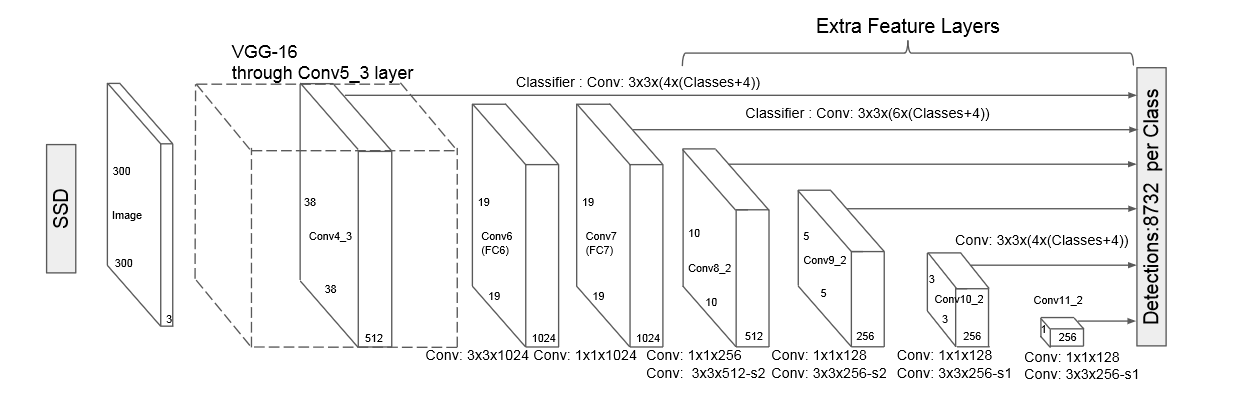
\includegraphics[width=0.8\linewidth]{SSD_Struture.png}
		\vspace{0.5cm}
		\captionof{figure}{Cấu tạo của một mạng SSD}
	\end{center}
	
	Sau khi có được các feature map, lớp Multibox sẽ tiến hành đưa ra dự đoán về ô bọc và nhãn gắn với ô bọc đó. Mỗi feature map sử dụng một tập hợp các lớp tích chập sẽ cho ra một số lượng dự đoán nhất định. Với mỗi vị trí trên feature map được kernel trượt qua, thì một dự đoán về ký tự được sinh ra. Kernel có kích thước:
	$$3 \times 3 \times (n \times (classes + 4))$$
	Với $n$ là số lượng tỉ lệ diện mạo với fearture map tương ứng và $classes$ là số lượng nhãn cần nhận diện, số $4$ trong công thức đại diện cho 4 thông số về vị trí của ô bọc (tọa độ trọng tâm và kích thước). Do kích thước của các kernel không đồng nhất (vì số lượng tỉ lệ diện mạo ứng với từng feature map có thể khác nhau), nên để tạo ra dữ liệu đầu ra phù hợp với các ô chuẩn đã tạo từ trước thì các vector dự đoán sẽ được sắp xếp lại sao cho dữ liệu đầu ra chỉ có $classes + 4$ kênh và vị trí của các vector phải tương ứng với vị trí các ô chuẩn đã sinh từ trước.
	
	\subsubsection{Tính giá trị mất mát}
	
	Giá trị mất mát được tính bằng tổng có trọng số giữa mất mát về vị trí\footnote{Thuật ngữ tiếng Anh: Localization Loss} và mất mát về độ tin cậy\footnote{Thuật ngữ tiếng Anh: Confidence Loss}
	
	$$ L(x,c,l,g) = \frac{1}{N} (L_{conf}(x,c) + \alpha L_{loc}(x,l,g) ) $$
	Trong đó:
	\begin{itemize}
		\item x biểu thị các phép kết hợp, cụ thể $x^p_{ij}$ biểu thị phép kết hợp giữa ô chuẩn thứ $i$ với ô bọc thứ $j$ đối với nhãn $p$. Vì vậy $x^p_{ij}$ có tập giá trị $\{0, 1\}$.
		\item $c$ biểu thị nhãn kỳ vọng cho phép kết hợp đang xét.
		\item $l$ biểu thị ô bọc dự đoán.
		\item $g$ biểu thị ô bọc "đáp án".
	\end{itemize}
	
	Hàm mất mát về vị trí có thể được biểu diễn bằng công thức:
	$$L_{loc}(x,l,g) = \sum^N_{i \in Pos} \sum_{m \in \{ cx, cy, w, g \}} x^k_{ij} smooth_{L1} (l^m_i - \hat{g}^m_j) $$
	Trong đó:
	\begin{itemize}
		\item N là số lượng phép kết hợp giữa ô chuẩn và ô bọc có ý nghĩa (nhãn của phép kết hợp không phải là "nền". Nếu như $N = 0$ thì ta đặt giá trị mất mát bằng 0.
		\item Pos là tập hợp các phép kết hợp có ý nghĩa.
		\item $smooth_{L1}$ là một hàm tính mất mát được định nghĩa là 
		$$L(x) = \begin{cases} 0.5x^2 \quad if |x| < 1 \\ |x| - 0.5 \quad otherwise \end{cases} $$
		\item $\hat{g}_j^{cx} = (g_j^{cx} - d_i^{cx}) / d^w_i$ Với $d$ biểu thị cho ô chuẩn.
		\item $\hat{g}_j^{cy} = (g_j^{cy} - d_i^{cy}) / d^h_i$
		\item $\hat{g}^w_j = \log \left( \frac{g_j^w}{d_i^w} \right)$
		\item $\hat{g}^h_j = \log \left( \frac{g_j^h}{d_i^h} \right)$
	\end{itemize}
	
	Vậy ta có thể thấy khi tính giá trại mất mát về vị trí, ta tính dựa trên sai lệch so với ô chuẩn mà ô bọc "đáp án" ban đầu kết hợp được thay vì tính mất mát trực tiếp.\\
	
	hàm mất mát về độ tin cậy có thể được tính theo công thức:
	
	\subsubsection{Bộ giải mã (Decoder)}
	
	Bản chất của bộ giải mã khá đơn giản, nó có chức năng chuyển dữ liệu các ô bọc mà mạng dự đoán (tức là những ô bọc được tính kích thước và tọa độ theo ô chuẩn mà ô bọc đó được kết hợp vào) sang dữ liệu tọa độ của ảnh (có gốc tọa độ nằm ở góc trên bên phải và tọa độ nằm trong miền $[0, 1]$
	
	\subsubsection{Một số vấn đề khác trong mạng SSD}
	\subsubsection*{Tăng cường dữ liệu\footnote{Data Augumentation}}
	
	Ngay trước quá trình kết hợp
	
	\subsubsection*{Cân bằng nhãn\footnote{Hard Negative Mining}}	
	%%%%%%%%%%%%%%%%%%%%%%%%%%%%%%%%%%%%%%%%%%%%%%%%%
	%%%%%%%%%%%%%%%%%%%%%%%%%%%%%%%%%%%%%%%%%%%%%%%%
	
	
	\newpage
	\section{Công trình liên quan}
	Là một phần quan trọng của hệ thống \textbf{Nhận dạng ký tự thuộc thị giác}\footnote{Thuật ngữ tiếng Anh: Optical Character Recognition, viết tắt OCR.}, nhận dạng \textbf{biểu thức toán học}\footnote{Thuật ngữ tiếng Anh: Mathematical Expression, viết tắt ME.} đã được nghiên cứu trong hơn nửa thế kỷ qua. Trên hành trình đó, rất nhiều công trình nhằm giải quyết vấn đề này đã được công bố. Trong chương này, nhóm sẽ trình bày tóm lược về một số công trình tiêu biểu, là những điểm tham khảo cho hệ thống nhận dạng biểu thức toán học mà nhóm sẽ hiện thực sau này và nhằm giúp cho bạn có một cái nhìn toàn cảnh về lĩnh vực này.
	\subsection{Cái nhìn toàn cảnh}
	
	Trong suốt hơn 50 năm hành trình, rất nhiều phương pháp nhận diện biểu thức toán học khác nhau đã được đề xuất, tuy vậy, bài toán này có thể được phân ra thành một số hướng tiếp cận khác nhau:
	
	\begin{itemize}
		\item Nhận diện theo hướng phân vùng\footnote{Thuật ngữ tiếng Anh: Segmentation.}. Ở hướng này, bài toán được chia ra thành nhiều bài toán nhỏ hơn thông qua việc phân chia vùng ảnh biểu thức toán học một cách có quy tắc. Một số ví dụ cho phương pháp này như giải thuật X-Y cut [trích dẫn] hay dùng phương pháp projection profiles. Đối với phương pháp này, bài toán sẽ trở nên vô cùng khó khăn với những ký tự dính liền nhau hoặc với những bài toán có dấu căn.
		
		\item Nhận diện dựa trên cấu trúc cây hoặc đồ thị. Ở hướng này, dựa vào vị trí các ký tự cũng như cấu trúc tổng thể của biểu thức, biểu thức toán học được biểu diễn theo cấu trúc cây hoặc đồ thị. Một số ví dụ cho phương pháp này như Tapia and Rojas Đã đề xuất một phương pháp nhận diện dựa trên cây trải dài\footnote{Thuật ngữ tiếng Anh: Spanning tree.} và ký tự chủ đạo\footnote{Thuật ngữ tiếng Anh: Dominate symbol.}, Zanibbi cho ra đời phương pháp nhận diện bằng một chuỗi các bước biến đổi cây. Phương pháp này khá hoàn thiện nhưng vẫn có một số vướng mắc như việc nhận diện ký tự một cách phi ngữ cảnh vẫn mang đến sự thiếu tự nhiên, hay phương pháp đọc từ trái sang phải vẫn để lại nhiều lỗ hổng trong việc nhận diện biểu thức.
		
		\item Nhận diện dựa trên ngữ pháp toán học. Ở hướng này, ngữ pháp được đưa vào quá trình nhận diện, ví dụ như sử dụng ngữ pháp để hậu xử lý, loại bỏ, hiệu chỉnh các ý tự nhận diện sai hoặc sử dụng các mô hình ngữ pháp để dự đoán ký tự tiếp theo trong biểu thức.
	\end{itemize}
	
	
	\subsection{WHOOOOOO ? \cite{zanibbi} : Watch, Attend and Parse: An End-to-end Neural Network Based Approach to Handwritten Mathematical Expression Recognition} 
	
	Khác với những bài báo đi trước sử dụng phương pháp phân vùng hay dựa trên ngữ pháp, bài báo này sử dụng phương pháp mang tên Watch, Attend, Parse dựa trên bài toán chú thích cho ảnh \footnote{Thuật ngữ tiếng anh: Image Captioning}. Hệ thống này là sự kết hợp giữa CNN, RNN và một hệ thống ANN (Cụ thể là GRU\footnote{Viết tắt: Gated recurrent unit}), CNN đặc trưng cho Watcher sẽ trích đặc trưng ảnh, ANN đặc trưng cho Attend mang nhiệm vụ điều hướng cho mạng biết được vị trí nào sẽ tập trung vào và RNN đặc trưng cho Parser mang nhiệm vụ sinh ra chuỗi Latex chính là đầu ra của hệ thống\\
	
	Cấu trúc mạng này được chia thành ba phần:
	\subsubsection{Watcher}
	Bộ phận này có bản chất là một hệ thống mạng nơ-ron tích chập đầy đủ (FCN)\footnote{Thuật ngữ tiếng anh: Fully Convolution Network} có cấu tạo là các lớp tích chập và các lớp pooling xếp chồng lên nhau. Bộ phận này nhận đầu vào là ảnh cần nhận diện và đầu ra là các vector đặc trưng ứng với mỗi pixel của ảnh.
	
	\subsubsection{Attend}
	Bộ phận này hoạt động giống như một hệ thống tổng hợp thông tin, nó có chức năng lấy dữ liệu ký tự vừa được dự đoán từ Parser (sẽ được giải thích bên dưới), từ các vector đặc trưng đã có được từ Watcher và ghi nhận các vị trí đã được xử lý trong ảnh, từ đó dự đoán vị trí tiếp theo để xử lý.
	
	\subsubsection{Parser}
	Bản chất của bộ phận này là một mạng GRU nhận dữ liệu đầu vào từ hai bộ phận còn lại, từ đó sinh ra chuỗi Latex
	
	\subsection{Wenhao He\cite{context}: Context-aware Recognition}
	\label{subsec: context}
	Một quá trình nhận dạng biểu thức toán học chuẩn bao gồm 2 giai đoạn: giai đoạn đầu tiên là phân tách và nhận dạng ký hiệu\footnote{symbol segmentation and recognition} , giai đoạn thứ hai là phân tích cấu trúc\footnote{structure analysis}. Nhiều công trình nghiên cứu trước đây về nhận dạng biểu thức toán học cũng thực hiện theo phương pháp như vậy. Nhược điểm của những phương pháp dạng này là thực hiện hai quá trình trên một cách độc lập, do đó thông tin cấu trúc\footnote{structure information hay context information} của biểu thức không được đưa vào quá trình nhận dạng. Như vậy sẽ dẫn đến lỗi\cite{context}.
	
	WenHao He cùng các cộng sự của ông đã đề xuất một phương pháp dựa trên CNN, kết hợp với cách học đa nhiệm vụ\footnote{multi-task learning}, cố gắng kết hợp hai giai đoạn chuẩn của quá trình nhận dạng biểu thức toán lại với nhau.
	
	Phương pháp mà các ông đưa ra đảm bảo thông tin cấu trúc của biểu thức được đưa vào quá trình nhận dạng và thể hiện trong các ma trận đặc trưng\footnote{feature map}\cite{yanlecun}. \\
	Đối với các phương pháp trước, biểu thức phải được phân tách thành những ký hiệu rồi từng ký hiệu này mới được đưa qua bộ nhận dạng. Một số phương pháp phân tách ký hiệu thường được sử dụng như: phân tích thành phần liên thông\footnote{connected components}, cắt dựa trên các phép chiếu\footnote{projection cutting}\cite{segment}. Tuy nhiên với phương pháp mới này, cả ảnh của biểu thức toán học được đưa qua bộ nhận dạng, chính vì vậy mà thông tin cấu trúc của biểu thức được bảo toàn. \\
	%\vspace{5cm}
	
	Dưới đây là mô hình học của phương pháp này:\\
	
	\begin{figure}[!h]
		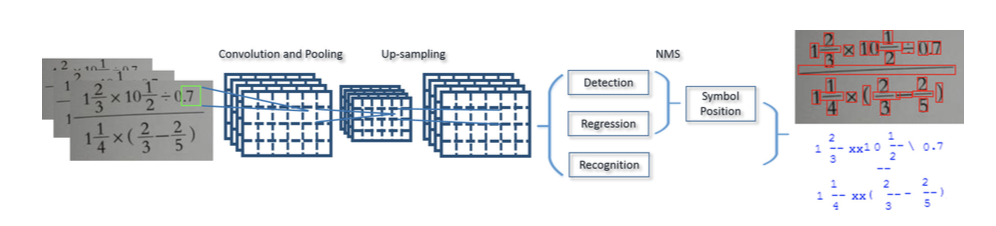
\includegraphics[]{context_aware.png}
		\vspace{0.2cm}
		\caption{Mô hình học được đề xuất \cite{context}.}
		
	\end{figure}
	
	Ảnh đầu vào sẽ qua một số lớp tích chập, down-sampling và up-sampling để tạo ra một feature map. Feature map này sẽ được gửi đến ba nhiệm vụ, mỗi nhiệm sẽ tạo ra 1 feature map có cùng kích thước với feature map đầu vào. \\
	Giả sử một điểm $i$ được cho đặt tại toạ độ ($w_i$, $h_i$) của feature map được tạo ra bởi các nhiệm vụ. 
	\begin{itemize}
		\item \textbf{Nhiệm vụ phát hiện} (Dectection task) sẽ cho ra một con số $s$ thể hiện độ tin cậy rằng một ký hiệu được đặt tại $i$.
		\item \textbf{Nhiệm vụ hồi quy} (Regression task) cho ra một vec-tor 4 chiều {$x_1$, $y_1$, $x_2$, $y_2$} thể hiện thông tin về bounding box của ký hiệu được đặt tại $i$.
		\item\textbf{Nhiệm vụ nhận dạng} (Recognition task) gán nhãn cho ký hiệu đặt tại $i$ cùng với xác suất của nhãn đó. 
	\end{itemize}
	
	Như vậy nhiệm vụ phát hiện và hồi quy được thiết kế để định vị trí của ký hiệu trong biểu thức toán học, nhiệm vụ nhận dạng quyết định xem đó là ký hiệu gì.
	
	Phương pháp nhận dạng như trên có thể giải quyết cả những trường hợp là thách thức đối với các phương pháp phân tách và nhận dạng ký hiệu trước đây, cụ thể đó là vấn đề gom nhóm ký hiệu đối với các ký hiệu nhiều phần nhỏ, tách những ký hiệu bị dính nhau.
	
	\subsection{QAK\cite{qak}}
	QAK là tên dự án được thực hiện bởi nhóm sinh viên khoá 2011 cũng về đề tài nhận dạng biểu thức toán học.
	
	Phương pháp nhóm sinh viên này xây dựng dựa trên nghiên cứu chính từ hai công trình của Aderson\cite{anderson} và Zanibbi\cite{zanibbi}. Do đó, qua trình nhận dạng biểu thức toán học vẫn đi theo 2 bước chuẩn đó là phân tách ký hiệu và phân tích cấu trúc như đã trình bày ở mục \ref{subsec: context}. 
	\newpage
	Dưới đây là mô hình phương pháp mà nhóm đã đề xuất:
	%\vspace{3cm}
	
	\begin{figure}[!h]
		\centering
		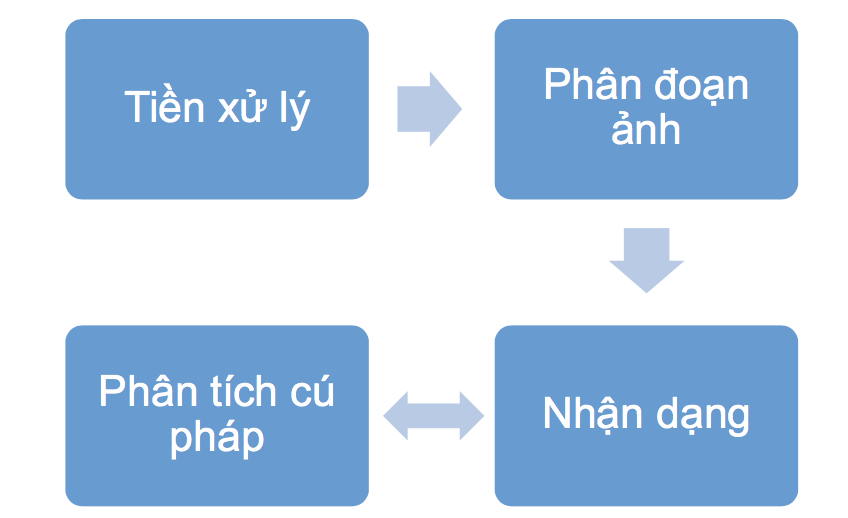
\includegraphics[width=0.5\linewidth]{2011.png}
		\vspace{1cm}
		\caption{Quy trình nhận dạng.}
		
	\end{figure}
	
	\begin{itemize}
		\item Trong bước tiền xử lý, nhóm áp dụng một số kỹ thuật trong xử lý ảnh như: loại nhiễu, ảnh nhị phân,... để tăng cường chất lượng ảnh, hỗ trợ cho bước phân đoạn.
		\item Trong bước phân đoạn ảnh, nhóm dùng kỹ thuật chính là cắt theo hình chiếu\cite{segment} và phân tích thành phần liên thông\cite{segment} cho toán tử lấy căn. Mục tiêu của giai đoạn này là phân tách ảnh chứa biểu thức toán học ban đầu ra thành các mảnh ảnh, mỗi mảnh chỉ chứa 1 ký hiệu toán học. Ngoài ra, ở bước này một cấu trúc cây được xây dựng lưu thông tin của các mảnh ảnh, hỗ trợ cho quá trình phân tích ngữ pháp sau này.
		\item Ở bước nhận dạng, nhóm sinh viên khoá 2011 đã sử dụng một kiến trúc mạng tương tự Lenet-5\cite{yanlecun}.
		\item Với phân tích cú pháp, nhóm sử dụng tập luật \textbf{văn phạm phi ngữ cảnh} \footnote{Thuật ngữ tiếng Anh: Context-free grammar} do chính nhóm đề xuất để giới hạn kết quả đầu ra của quá trình nhận dạng, từ đó tăng khả năng nhận dạng đúng biểu thức. 
	\end{itemize}
	
	%%%%%%%%%%%%%%%%%%%%%%%%%%%%%%%%%%%%%%%%%
	%%%%%%%%%%%%%%%%%%%%%%%%%%%%%%%%%%%%%%%%%
	
	\newpage
	\section{Mô hình đề xuất}
	
	\subsection{Tổng quan}
	
	Nhóm quyết định sử dụng mạng SSD\footnote{Thuật ngữ tiếng Anh: Single Shot Detector} để phát hiện các ký tự trong ảnh và sau đó sử dụng bộ phân tích cú pháp DRACULAE để sinh ra chuỗi Latex.
	
	\subsection{Phát hiện ký tự}
	
	\subsubsection{Mạng cơ sở}
	
	Về cấu trúc của SSD, nhóm đã sử dụng mạng VGG16 [trích dẫn] cho phần mạng cơ sở. Cấu trúc của mạng VGG16 gồm tổ hợp các lớp tích chập và lớp pooling xếp chồng lên nhau, ở cuối mạng có các lớp liên kết đầy đủ \footnote{Thuật ngữ tiếng Anh: Fully connected layer} để giảm kích thước tensor và cuối cùng là xuất ra vector có số chiều phù hợp (có số chiều bằng với số lớp đối tượng cần dự đoán).
	
	\begin{center}
		
		\centering
		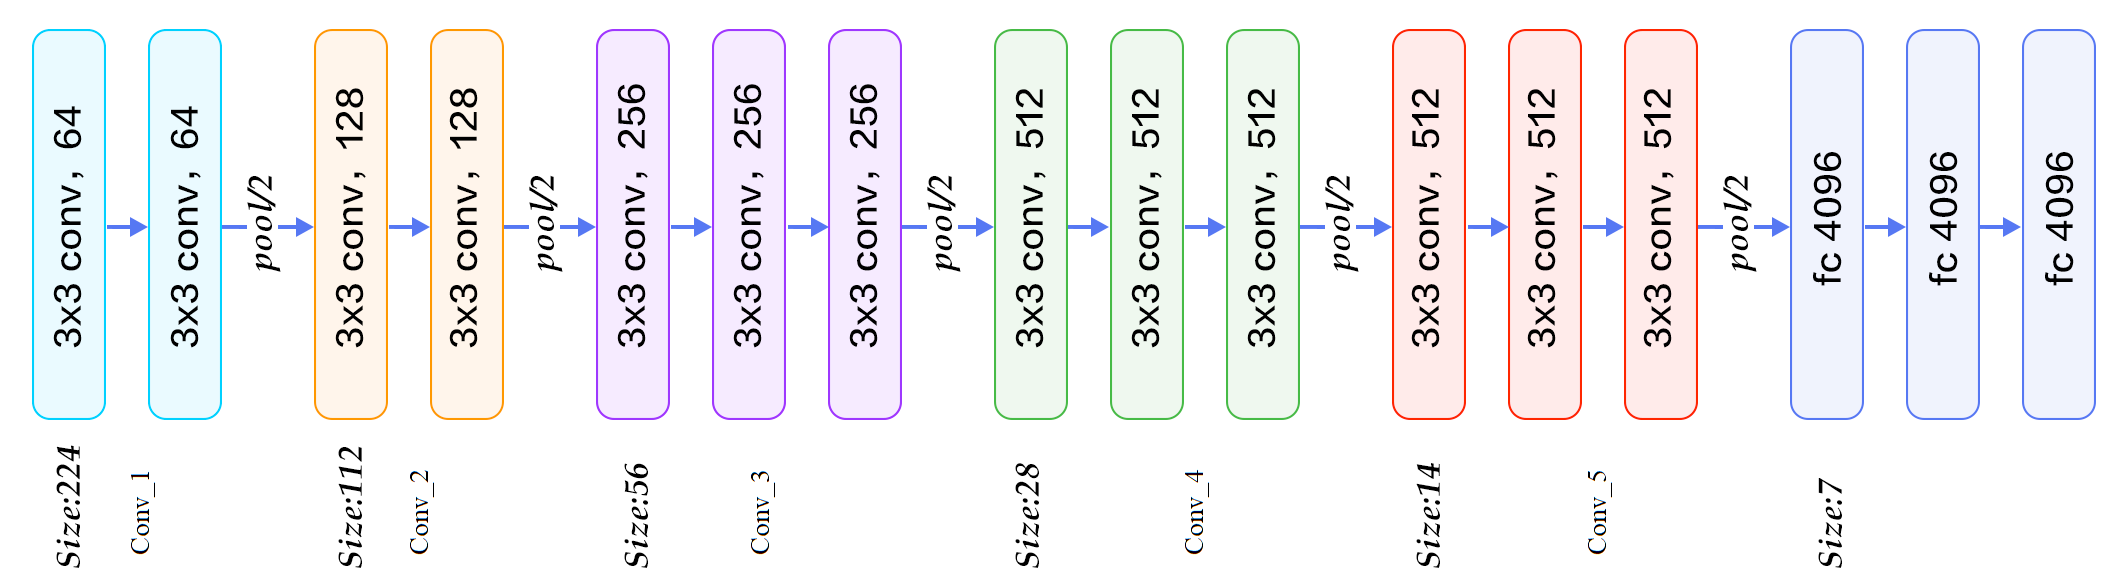
\includegraphics[width=0.8\linewidth]{vgg16.png}
		\vspace{0.5cm}
		\captionof{figure}{Cấu tạo mạng VGG16}
	\end{center}
	
	Như hình vẽ bên trên, các lớp tích chập và lớp pooling được gom lại thành các cụm, sau hai đến ba lớp tích chập là một lớp pooling. Số kênh của tensor chạy trong mạng được nâng dần từ 64 lên 512 về phía cuối mạng. Khi đưa mạng cơ sở vào mạng SSD, các lớp liên kết đầy đủ sẽ được bỏ đi và bộ phận phân loại sẽ được chèn vào vị trí tương ứng. Khi đó, ta cần phải chuyển model của mạng VGG sang mạng SSD, phần này sẽ được đề cập chi tiết hơn trong phần hiện thực.
	
	\subsubsection{Thân mạng SSD}
	
	Khi tiếp hợp vào mạng SSD, các lớp liên kết đầy đủ của VGG16 được lược bỏ, thay vào đó là những lớp tích chập, mô hình cụ thể của mạng SSD nhóm để xuất được thể hiện ở ảnh dưới.
	
	\begin{center}
		
		\centering
		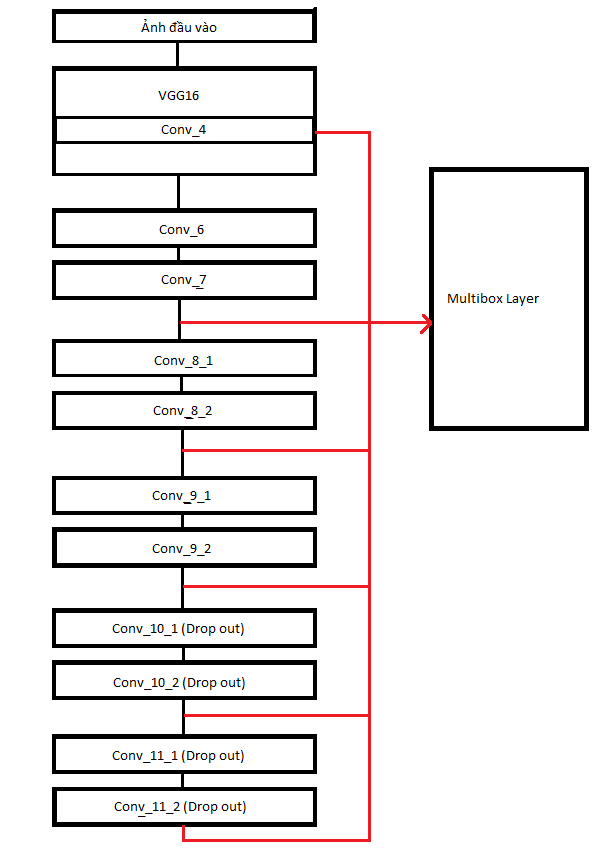
\includegraphics[width=0.8\linewidth]{SSD_Layers.png}
		\vspace{0.5cm}
		\captionof{figure}{Sơ đồ các lớp trong mạng SSD}
	\end{center}
	
	Trong đó Khối VGG16 là phần mạng VGG16 đã được lược bỏ các lớp liên kết đầy đủ. Các khối còn lại được thể hiện trong bảng sau:
	
	\begin{center}
		\begin{tabular}{||c | c | c | c | c | c ||} 
			\hline
			Khối & \makecell{ Số kênh \\ đầu vào } & \makecell{ Số kênh \\ đầu ra} & Kích thước nhân &  \makecell{ Chèn thêm \\ (Padding) } &  \makecell{ Bước \\ (Stride) } \\ [0.5ex] 
			\hline\hline
			Conv\_6 & 512 & 1024 & 3 & 1 & 1 \\ 
			\hline
			Conv\_7 & 1024 & 1024 & 3 & 6 & 1 \\ 
			\hline
			Conv\_8\_1 & 1024 & 256 & 1 & 0 & 1 \\ 
			\hline
			Conv\_8\_2 & 256 & 512 & 3 & 1 & 2 \\ 
			\hline
			Conv\_9\_1 & 512 & 128 & 1 & 0 & 1 \\ 
			\hline
			Conv\_9\_2 & 128 & 256 & 3 & 1 & 2 \\ 
			\hline
			Conv\_10\_1 & 256 & 128 & 1 & 0 & 1 \\ 
			\hline
			Conv\_10\_2 & 128 & 256 & 3 & 1 & 2 \\ 
			\hline
			Conv\_11\_1 & 256 & 128 & 1 & 0 & 1 \\ 
			\hline
			Conv\_11\_2 & 128 & 256 & 3 & 0 & 1 \\ 
			\hline
		\end{tabular}
	\end{center}
	
	Riêng khối Conv\_4 trong ảnh là lớp tích chập thứ 10 trong mạng VGG.\\
	
	Các lớp tích chập đều sử dụng hàm truyền là hàm ReLu, riêng ở sau các lớp Conv\_10\_1, Conv\_10\_2, Conv\_11\_1, Conv\_11\_2 thì có thêm một lớp dropout với hệ số dropout là 0.2.
	
	Các feature map được trích ra để thực hiện phát hiện, phân loại từ các mủi tên màu đỏ trên hình, cụ thể:
	
	\begin{itemize}
		\item Ngay sau khối tích chập - pooling 512 thứ nhất trong mạng VGG (hay sau lớp pooling của lớp tích chập thứ 10 của mạng VGG - hay Conv\_4).
		\item Sau các khối tích chập Conv\_7, Conv\_8, Conv\_9, Conv\_10, Conv\_11.
	\end{itemize}
	
	Đối với mạng SSD300[trích dẫn] nguyên thủy, kích thước của các feature map ứng với số dự đoán được thể hiện ở bảng sau:
	
	\begin{center}
		\begin{tabular}{||c | c | c | c ||} 
			\hline
			\makecell{ Feature map \\ Sinh bởi } & \makecell{ Kích thước} & \makecell{Tỉ lệ \\ diện mạo } &  \makecell{ Số dự đoán } \\ [0.5ex] 
			\hline\hline
			Conv\_4 & $512 \times 38 \times 38$ & $ \{ 1, \frac{1}{2} , 2\} $ & 5776 \\ 
			\hline
			Conv\_7 & $1024 \times 19 \times 19$ & $ \{ 1, \frac{1}{2} , 2, \frac{1}{3}, 3\} $ & 2166 \\ 
			\hline
			Conv\_8 & $512 \times 10 \times 10$ &  $ \{ 1, \frac{1}{2} , 2, \frac{1}{3}, 3\} $ & 600 \\ 
			\hline
			Conv\_9 & $256 \times 5 \times 5 $ &  $ \{ 1, \frac{1}{2} , 2, \frac{1}{3}, 3\} $ & 150  \\ 
			\hline
			Conv\_10 & $256 \times 3 \times 3$ & $ \{ 1, \frac{1}{2} , 2\} $ & 36 \\ 
			\hline
			Conv\_11 & $256 \times 1 \times 1$ & $ \{ 1, \frac{1}{2} , 2\} $ & 4 \\ 
			\hline
		\end{tabular}
	\end{center}
	
	Như vậy, ứng với mỗi ảnh, hệ thống sinh ra 8732 dự đoán. Tương ứng, bộ phận mã hóa của mạng SSD300 cũng có những thông số:
	
	\begin{itemize}
		\item Danh sách kích thước feature map: (38, 19, 10, 5, 3, 1)
		\item Danh sách kích thước các ổ chuẩn (với $s_{min} = 0.2$ và $s_{max} = 0.9$): (30, 60, 111, 162, 213, 264, 315)
		\item Ngưỡng Jaccard: 0.5.
	\end{itemize}
	
	\subsubsection{Các thay đổi}
	
	Do bản chất mạng SSD300 gặp rất nhiều khó khăn trong việc nhận dạng ký tự nhỏ do một số lý do:
	\begin{itemize}
		\item Trong quá trình kết hợp, các ô bọc "đáp án" kết hợp với ô chuẩn phải có chỉ số Jaccard lớn hơn 0.5, nhưng kích thước tối thiểu của ô chuẩn lại là $30 \times 30$ pixel, vì vậy nhiều ký tự nhỏ không thể kết hợp được (Trường hợp này xãy ra với hầu hết những ảnh có chữ nhỏ, ví dụ như ảnh dưới)
		\begin{center}
			\centering
			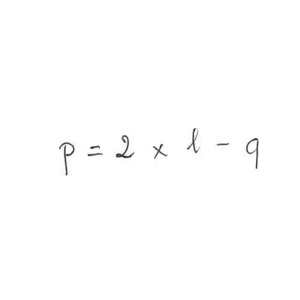
\includegraphics[resolution=300]{HMER_2017_TEST1_MINH_01_2A.png}
			\vspace{0.5cm}
			\captionof{figure}{Ảnh ví dụ chữ nhỏ (với kích thước thật)}
		\end{center}
		Khi không thể kết hợp được thì vùng ký tự đó được hiểu là phần nền, điều này gây bất lợi lớn cho quá trình huấn luyện do vùng ảnh không trống nhưng lúc là nền lúc lại được gắn nhãn.
			
		\item Nhiều ký tự có tỉ lệ diện mạo đặc biệt (Ví dụ như ký tự dấu $-$ trong phân số hoặc $\int$) cũng gặp nhiều khó khăn trong việc kết hợp do không đạt được ngưỡng Jaccard.
	\end{itemize}
	
	Vì vậy, nhóm đã sửa một số thông số để tìm cách giải quyết vấn đề trên, trong nhiều bộ thông số thì có 3 mô hình nổi bật.
	
	\subsubsection*{Giảm kích thước các ô chuẩn}
	
	Mô hình này dựa trên mô hình SSD300 nguyên thủy, chỉ chỉnh sửa kích thước các ô bọc thông qua chỉnh hai thông số $s_{min} = 0.08$ và $s_{max} = 0.5$, từ đó danh sách kích thước các ô chuẩn được thay đổi thành (9, 24, 54, 84, 114, 144, 174). So với mô hình nguyên thủy, mô hình này không thể kết hợp tốt các ký tự lớn (lớn hơn khoảng $200 \times 200$ pixel). Tuy vậy, đối với bài toán về phát hiện các ký tự trong một ảnh, thì kích thước các ký tự không thể quá lớn, nên những ký tự đặc biệt lớn như vậy có thể được xem xét ở độ ưu tiên thấp hơn.\\
	
	Việc thay đổi tham số ở mô hình này không làm ảnh hưởng lớn đến cấu trúc mạng cũng như quá trình mã hóa, giải mã. Số lượng dự đoán không thay đổi.\\
	
	Mục đích chính của thay đổi này là để quá trình kết hợp diễn ra tốt hơn khi kích thước của ô chuẩn nhỏ nhất là $9 \times 9$, điều này 
	
	\subsubsection*{Giảm kích thước các ô chuẩn và tăng kích thước ảnh đầu vào}
	
	Ở mô hình này
	
	\subsection{Phân tích cú pháp}
	
	Bộ phân tích cú pháp này có nhiệm vụ chuyển dữ liệu dự đoán là các ô bọc sang dữ liệu biểu thức toán học dạng latex.\\
	
	\subsubsection{Sinh cây BST}
	
	Đây là giai đoạn phức tạp nhất và cũng là quan trọng nhất, ở giai đoạn này, dữ liệu đầu ra từ mạng SSD là danh sách các ô bọc sẽ được phân tích và xây dựng một cây BST. Công việc này có thể được phân ra thành bốn công đoạn: Tìm ký tự chủ đạo, xác định những ký tự trên đường cơ sở, tái phân vùng và đệ quy\\
	
	Trước khi tiến hành sinh cây, ta cần phải phân loại các ký tự vào những thể loại khác nhau, điều này có mục đích giúp xác định vị trí trọng tâm tốt hơn, xác định được vùng ảnh gắn với chỉ số trên, chỉ số dưới và giúp phân biệt một số loại ký tự có thể có cấu trức đặc biệt trong biểu thức (ví dụ như ký tự $\sum$ thì có thể có ký tự nằm trên và bên dưới, nhưng ký tự $sin$ thì gần như không bao giờ có). Các ký tự được phân vào các lớp như bảng dưới:
	
	\begin{center}
		\begin{tabular}{||c | c | c c c c ||} 
			\hline
			Lớp ký tự & Tung độ trọng tâm & Bên dưới & Bên trên & Chỉ số dưới & Chỉ số trên \\ [0.5ex] 
			\hline\hline
			\makecell{Non-Script \\ Các ký tự phép tính\\ $(+, -, \rightarrow, ... )$} & $\frac{1}{2}H$ & $\frac{1}{2}H$ & $\frac{1}{2}H$ & - & - \\ 
			\hline
			\makecell{Open Bracket \\ Ký tự mở ngoặc \\ ( } & $cH$ & $min(Y)$ & $max(Y)$ & - & - \\
			\hline
			\makecell{Root \\ Ký tự căn \\ $\sqrt{}$ } & $cH$ & $min(Y)$ & $max(Y)$ & $tH$ & $H - tH$ \\
			\hline
			\makecell{Variable Range \\ Ký tự có thể viết \\ ở trên hoặc dưới \\ $\sum$, $\int$, $\lim$ ... } & $\frac{1}{2}H$ & $tH$ & $H-tH$ & $tH$ & $H- tH$ \\
			\hline
			\makecell{Ascender \\ Ký tự nổi lên \\ A..Z, 0..9, b,d,f ... } & $cH$ &  $tH$ & $H-tH$ & $tH$ & $H- tH$ \\
			\hline
			\makecell{Descender \\ Ký tự chìm xuống \\ g, p, y, j, ..., b,d,f ... } & $H - cH$ &  $\frac{1}{2}H + t\frac{1}{2}H$ & $H-t\frac{1}{2}H$ & $\frac{1}{2}H + t\frac{1}{2}H$ & $H-t\frac{1}{2}H$ \\ 
			\hline
			\makecell{Centered \\ Ký tự trung tâm \\ o, n, u, \}, ) ... } & $\frac{1}{2}H$ &  $tH$ & $H-tH$ & $tH$ & $H- tH$
			\\ \hline
			
			
		\end{tabular}
	\end{center}
	
	Trong đó:
	\begin{itemize}
		\item Các cột thứ hai trở đi là tọa độ của một số điểm, ngưỡng đặc biệt tính từ góc trái bên dưới của ký tự. Hệ trục tọa độ có trục tung hướng lên và trục hoành hướng sang phải. Cột "Tung độ trọng tâm" thể hiện tung độ y của trọng tâm của ký tự, cột bên dưới và bên trên thể hiện ngưỡng trên và ngưỡng dưới của ký tự, các ký tự vượt ngoài ngưỡng đó sẽ được xem là nằm bên trên hoặc nằm bên dưới ký tự đang xét (Ví dụ như một ký tự nào đó có tung độ trọng tâm lớn hơn $max(Y)$ của môt ký tự thuộc lớp $Root$ thì sẽ được xem là nằm bên trên). Cột chỉ số trên, chỉ số dưới thể hiện ngưỡng để được phân vào vùng chỉ số trên, chỉ sô dưới. Riêng hai lớp Non-scipt và Open Bracket có giá trị hai cột này không xác định là do những ký tự của lớp này không có chỉ số trên, dưới.
		\item $H$ là chiều cao của ký tự.
		\item $c$ (Viết tăt của centroid ratio): là tham số để xác định trọng tâm cho một số ký tự đặc biệt (ví dụ như các ký tự ngoặc hoặc chìm xuống dưới), tùy người viết chữ có thể có những giá trị phù hợp khác nhau.
		\item $t$ Là ngưỡng cho chỉ số trên, dưới và chỉ phần bên trên, bên dưới. Tham số này biểu thị sự nhạy cảm đối với những ký tự trên dưới, tham số này càng lớn thì các ký tự khi được phân tích vị trí càng dễ được xếp vào chỉ số trên, chỉ số dưới.
	\end{itemize}
	
	Bảng trên thể hiện quy tắc để kiểm tra hai ký tự có vị trí tương đối như thế nào với nhau, cụ thể:
	\begin{itemize}
		
		\item B chứa trong A (dành cho trường hợp ký tự căn: $\sqrt{}$) khi B có tung độ nằm trong khoảng từ ngưỡng chỉ số dưới đến ngưỡng chỉ số trên của A và hoành độ trọng tâm của B nằm trong khoảng $(Min(X_B), Max(X_B)$.
		
		\item A và B liền kề nếu như trọng tâm của B có tung độ nằm trong khoảng từ ngưỡng chỉ số dưới đến ngưỡng chỉ số trên của A và hoành độ trọng tâm của B lớn hơn $Max(X_A)$.
		
		\item B là chỉ số trên của A nếu như trọng tâm của B lớn hơn ngưỡng chỉ số trên của A.
		
		\item B là ký tự phân số thống trị A khi trọng tâm của A có hoành độ nằm trong khoảng $(Min(X_B), Max(X_B)$
		
	\end{itemize}
	
	Trước khi tiến hành sinh cây BST, danh sách ô bọc cần phải được sắp xếp theo chiều tăng dần hoành độ của mép phải ô bọc $x$ (hay cụ thể hơn là $min(x)$). \\
	
	\subsubsection*{Tìm ký tự chủ đạo}
	
	Trong hầu hết trường hợp, ký tự chủ đạo là ký tự nằm bên trái nhất, tuy vậy, ta vẫn cần phải kháng được những trường hợp người dùng viết chữ không chuẩn gây thụt ra ngoài, hoặc những ký tự có dạng như:
	
	$$ \sum^{n = 100000} a $$
	Thì ký tự chủ đạo là $\sum$ nhưng ký tự bên trái nhất lại là $n$, Draculae được thế kế để có thể chống lại những trường hợp như vậy.\\
	
	Để tìm ký tự chủ đạo, ta cần thực hiện những công đoạn sau:
	\begin{itemize}
		\item Trước hết, ta tìm ký tự nằm bên trái nhất dựa trên $min(X)$ của ô bọc, xem tất cả các ký tự là nút con của nút gốc.
		\item Kiếm tra ký tự hiện tại có phải là Variable Range (lớp này có đặc tính có thể viết cả ở bên trên và bên dưới, đây là nguồn gốc gây khó khăn trong việc xác định ký tự chủ đạo). Nếu đúng thì ta kiểm tra xem ký tự đó có bị thống trị bởi một phân số hay không, nếu có thì ký tự chủ đạo là ký tự phân số, nếu không thì ký tự chủ đạo là ký tự Variable Range vừa tìm được. Nếu ký tự vừa tìm được không phải là Variable Range, thì ta tìm kiếm ký tự Variable Range nằm bên trái nhất và sang bước tiếp theo.
		
		\item Nếu không còn ký tự Variable Range nào khác, thì ký tự bên trái nhất vừa tìm được ở bước trên được kiểm tra bị thống trị bởi phân số hay không và trả về ký tự chủ đạo (ký tự đó hoặc ký tự phân số). Nếu còn một ký tự Variable Range khác trong biểu thức, ta tiếp tục với bước kế tiếp.
		
		\item Ta kiểm tra xem ký tự Variable Range khác đó có ký tự nào nằm liền kề bên trái không. Nếu không thì tự Variable Range được kiểm tra xem có bị thống trị bởi ký tự phân số hay không và chọn ký tự chủ đạo ký tự phù hợp. Nếu tồn tại ký tự liền kề bên trái, thì ký tự bên trái nhất được kiểm tra có bị thống trị bởi phân số không và chọn ký tự chủ đạo phù hợp.
		
	\end{itemize}
	
	\subsubsection*{Xác định ký tự trên đường cơ sở}
	
	Sau khi đã có được ký tự chủ đạo, ta cần phải tìm những ký tự liền kề theo chiều ngang với ký tự vừa tìm được, những ký tự này chính là ký tự trên đường cơ sở. Để xác định các ký tự trên đường cơ sở, ta lấy ký tự chủ đạo vừa xác định được để xét:
	
	\begin{enumerate}
		\item Nếu như ký tự đang xét là ký tự cuối cùng hoặc ký tự duy nhất được xét, thì chuyển sang bước kế tiếp (bước tái phân vùng).
		\item Ta phần vùng các ký tự nằm ở vùng bên trên, bên dưới, góc trên bên trái và góc dưới bên trái (không phân vùng các ký tự nằm bên phải) vào nút con của nút đang xét.
		\item Nếu như ký tự đang xét thuộc lớp Non-script, ký tự đó được đánh dấu nằm trên đường chủ đạo, ta quay lại tìm ký tự chủ đạo trong các ký tự còn lại và xác định các ký tự trên đường cơ sở với ký tự chủ đạo đó (quay lại bước 1).
		\item Ta kiểm tra danh sách các ký tự còn lại xem có ký tự nào liền kề bên phải với ký tự đang xét hay không, nếu có, ta kiểm tra ký tự đó có bị thống trị bởi ký tự khác hay không và quay lại bước 1 với ký tự được xét là ký tự thống trị nhất (hoặc chính ký tự liền kề nhất vừa tìm được đối với trường hợp nó không bị thống trị bởi ký tự nào).
		\item Nếu hệ thống chạy đến bước này thì có nghĩa là trong các ký tự còn lại, không còn ký tự nào liền kề với ký tự đang xét, vì vậy ta tiến hành phân vùng đưa các ký tự còn lại vào nút con góc trên bên phải (chỉ số trên) và góc dưới bên phải (chỉ số dưới) của nút đang xét.
	\end{enumerate}
	
	Sau khi thực hiện bước này lần đầu tiên, ta thu được một cây có ba tầng, tầng đầu chứa nút gốc, tầng thứ hai chứa các ký tự nằm trên đường cơ sở, tầng thứ ba chứa các nút con của các nút chứa ký tự nằm trên đường cơ sở, các nút con này có thể chứa một hoặc nhiều ký tự, chưa là một cây.
	
	\subsubsection*{Tái phân vùng}
	Ở bước trước, nút con được phân vào vùng góc trên bên trái và góc dưới bên trái, điều này không có ý nghĩa đối với ngữ nghĩa của biểu thức toán học và khó khăn trong việc sinh cây Lexed BST sau này. Vì vậy ở bước này, các nút con sẽ được thay đổi vị trí cho phù hợp với ngữ nghĩa của biểu thức, chương trình sẽ kiểm tra từng cặp ký tự liền kề theo thứ tự từ trái sang phải, ta gọi ký tự bên trái là $A$ và ký tự bên phải là $B$:\\
	
	\begin{itemize}
		\item Nếu $B$ không thuộc lớp Variable Range, và $B$ không có nút con ở vùng bên trên, ta gắn nút góc trên bên trái của ký tự $B$ vào nút góc trên bên phải (chỉ số trên) của $A$. 
		\item Nếu $B$ thuộc lớp Variable Range thì ta sẽ phân vùng những ký tự liền kề với ký tự đầu tiên trong nút con góc trên bên trái của $B$ vào vùng bên trên của $B$. 
		\item Nếu $A$ thuộc lớp Variable Range thì ta phải tiến hành gộp các vùng góc trên bên trái, bên trên và góc trên bên phải thành một vùng bên trên duy nhất.
	\end{itemize}
	
	Sau đó ta tiến hành làm tương tự với vùng bên dưới. Với cách phân vùng này, với một số biểu thức đặc biệt hoặc nhập nhằng thì việc phân vùng sẽ không chính xác, để khắc phục điều này, ta cần phải có thêm công đoạn hậu xử lý.\\
	
	\subsubsection*{Đệ quy}
	
	Tới bước này, ta đã có một cây có ba tầng với tầng thứ hai có phân vùng nút con khá chuẩn xác. Nhiệm vụ bây giờ là phải tiếp tục phân vùng cho các nút con của các ký tự trên đường cơ sở. Việc này được thực hiện bằng cách xem từng nút con là từng vùng ảnh mới riêng biệt và thực hiện lại ba bước trên để thu được các cây con. \\
	
	Sau quá trình này, ta thu được một cây BST biểu thị vị trí tương đối giữa các nút. Cây này tiếp tục được đi qua [Lexical Pass] để thu được Lexed - BST.
	
	\subsubsection{Sinh cây Lexed - BST}
	
	Sau khi đã thu được cây BST từ danh sách các ô bọc, nhiệm vụ còn lại là không quá phức tạp. Trước khi tạo được chuỗi Latex, ta cần phải sinh ra được một cây Lexed - BST, cây này chứa các thông tin như "nhóm ký tự" và cấu trúc biểu thức:
	
	\begin{itemize}
		\item Nhóm ký tự: Ban đầu, các ký tự được gom thành từng nhóm có nghĩa (Ví dụ các ký tự "s", "i", "n" thì sẽ được gộp lại thành một ký tự "sin" duy nhất.
		\item Ta sử dụng các luật khác nhau để sinh ra cây Lexed - BST.
	\end{itemize}
	
	\subsubsection*{Luật sinh}
	

	Để chuyển từ cây BST sang cây lexed - BST, nhóm có đề xuất một số luật sinh: \\
	Gọi ký tự đang xét là $A$
	\begin{itemize}
		\item Nếu cây BST $B$ nằm trong nút con góc phải bên dưới của $A$ thì sinh ra một nút sub(A, B)
		\item Nếu cây BST $B$ nằm trong nút con góc phải bên trên của $A$ thì sinh ra một nút sup(A, B)
		\item Nếu cây BST $B$ nằm trong nút con bên trong của $A$ và $A$ là ký tự căn ($\sqrt{}$) thì sinh ra một nút sqrt(B)
		\item Nếu $A$ có nút con bên trên hoặc bên dưới (hoặc cả hai), thì tùy thuộc vào ký tự $A$ mà ta sinh ra các nút khác nhau (Ví dụ như các ký tự $\sum$, $\lim$, $\prod$ , $\int$, $\rightarrow$ và quan trọng nhất là dấu gạch ngang trong phân số)
		
	\end{itemize}
	
	Sau khi sinh được cây Lexed - BST, hệ thống sẽ duyệt qua cây theo chiều tiền thứ tự để sinh mã Latex
	
	%%%%%%%%%%%%%%%%%%%%%%%%%%%%%%%%%%%%%
	%%%%%%%%%%%%%%%%%%%%%%%%%%%%%%%%%%%%%
	
	\section{Hiện thực, đánh giá}
	
	Để xây dựng hệ thống nhận diện biểu thức toán học viết tay, nhóm cần hoàn thành ba công việc chính bao gồm thu thập dữ liệu, huấn luyện mạng SSD và xây dựng chương trình sinh mã latex.
	
	\subsection{Chuẩn bị dữ liệu}
	
	\subsection{Hiện thực hệ thống}
	
	\subsubsection{Quá trình tiền huấn luyện}
	Như đã trình bày ở trên, mạng SSD mà nhóm lựa chọn có sử dụng mạng cơ sở là VGG16, đây là một mạng phân lớp\footnote{Thuật ngữ tiếng anh: Classification}. Để đạt được kết quả huấn luyện cho mạng SSD tốt hơn, tác giả đã khuyến cáo sử dụng phương pháp học chuyển tiếp\footnote{Thuật ngữ tiếng anh: Transfer Learning}
	
	\subsubsection*{Học chuyển tiếp}
	
	Để thực hiện phương pháp này, ta cần phải chuẩn bị một tập dữ liệu riêng gồm các ảnh ... <<<<<<<<<<<<<<<<<<<<\\
	
	Khi đã thu được một mô hình phù hợp (Huấn luyện tập tiền huấn luyện đã hội tụ), nhiệm vụ kế tiếp là ta phải chuyển các tham số đã học được sang một mô hình của mạng SSD.\\
	
	Quá trình này không quá phức tạp, nhóm đã viết một đoạn mã giúp tạo một mô hình mạng SSD rỗng, sau đó gán tham số từ mô hình mạng VGG16 vừa thu được sang mô hình mạng SSD mới. Ta bỏ qua các lớp liên kết đầy đủ do phần này đã được lược bỏ, lớp pooling cũng được bỏ qua do lớp này không có tham số. \\
	
	Sau khi đã thu được mô hình mạng SSD, ta có thể bước tiếp đến công đoạn huấn luyện mạng SSD.
	
	\subsection{Xây dựng chương trình sinh mã latex}
	
	
	\section{Tổng kết}
	\subsection{Công việc đã làm được}
	\subsubsection{Chuẩn bị cơ sở lý thuyết}
	
	\begin{itemize}
		\item Hiểu được luận văn của nhóm sinh viên khóa 2011 ở mức độ hiện thực lại được.
		\item Tìm hiiểu về mạng CNN ở mức độ hiểu được quy tắc truyền xuôi và truyền ngược.
		\item Đã tìm hiểu được cách hiện thực mạng CNN của caffe.
		\item Đọc và hiểu được các phương pháp giải quyết cho vấn đề nhận dạng biểu thức toán học được nêu trong các công trình nghiên cứu gần đây nhất.
		
	\end{itemize} 
	
	\subsubsection{Xây dựng bản thử nghiệm}
	
	Nhóm đã thử viết lại một bản demo để nhận diện một số biểu thức đơn giản theo giải thuật của nhóm sinh viên khóa 2011. Dữ liệu sử dụng là tập các hình ảnh được thu thập và xử lý trong đề tài nhận dạng biểu thức toán học của nhóm sinh viên trên.
	
	Ảnh dưới: cây cú pháp nhóm đã xây dựng được từ hình ảnh biểu thức toán học, và các số trong ô màu đỏ chính là ký tự mà hệ thống đoán được.\par
	
	\begin{center}
		
		\centering
		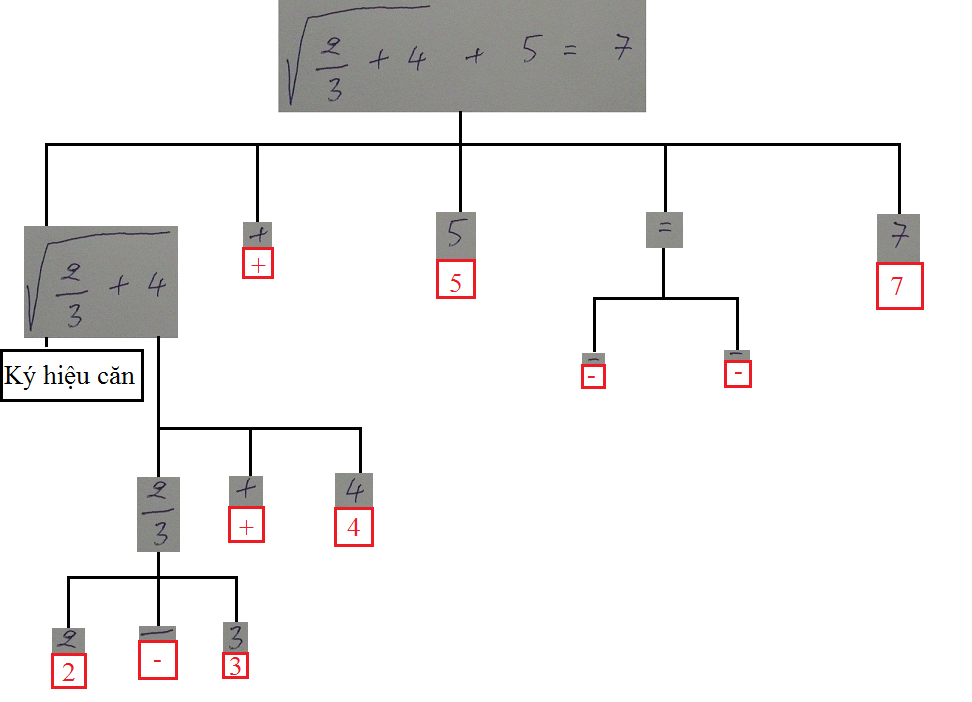
\includegraphics[width=0.8\linewidth]{kq_1_1.png}
		\vspace{0.5cm}
		\captionof{figure}{Sơ đồ mô tả kết quả demo 1}
	\end{center}
	
	\newpage
	\begin{center}
		
		\centering
		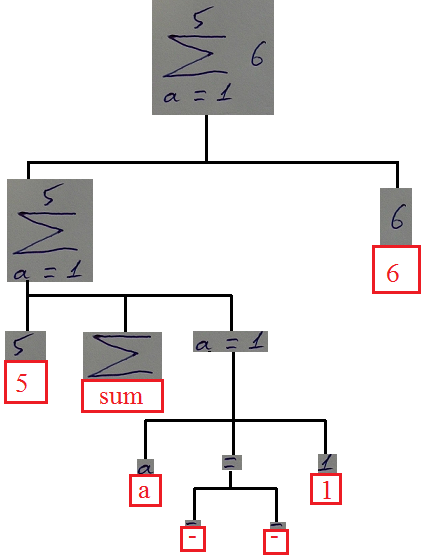
\includegraphics[width=0.8\linewidth]{kq_2_1.png}
		\vspace{0.5cm}
		\captionof{figure}{Sơ đồ mô tả kết quả demo 2}
	\end{center}
	\vspace{0.5cm}
	\subsection{Nhận xét bản thử nghiệm hiện tại}
	
	Một số vấn đề còn tồn đọng: 
	\begin{itemize}
		\item Khi nhận diện các ký tự toán học, hệ thống chưa phân biệt được ký tự chuẩn và các chỉ số.
		\item Nhược điểm lớn nhất của hệ thống là không thể phân tách được các ký tự dính liền nhau.
		\item Hệ thống không thể nhận diện các ảnh có nhiễu lớn.
	\end{itemize}
	
	Đây cũng là vấn đề chưa giải quyết được trong luận văn của nhóm sinh viên khoá 2011.
	\subsection{Kế hoạch trong giai đoạn tới}
	Vì những nhược điểm kể trên của phương pháp hiện tại, cộng với gợi ý hướng đi của giáo viên hướng dẫn, nhóm quyết định sử dụng một hướng tiếp cận mới.
	Ở giai đoạn tiếp đến, nhóm có kế hoạch:
	\begin{itemize}
		\item Trong tháng đầu của giai đoạn hè: Tìm hiểu về các phương án và chốt phương án hiện thực.
		\item Trong phần còn lại của giai đoạn hè và tháng đầu của giai đoạn luận văn (tuần 1 đến tuần 4): Vừa tìm hiểu về phương án vừa tiến hành hiện thực một số module cơ bản.
		\item Trong tháng kế tiếp (tuần 5 đến tuần 8): Củng cố cơ sở lý thuyết, tiến hành huấn luyện mạng và bắt đầu thiết kế demo.
		\item Trong tháng kế tiếp (tuần 9 đến tuần 13): hiện thực demo và tiến hành lên sản phẩm (trước hội nghị tháng 10).
		\item Thời gian còn lại tiến hành hiệu chỉnh tham số để thử nghiệm độ hiệu quả, sửa lỗi trong hệ thống và viết báo cáo.
	\end{itemize}
	
	
	
	\newpage
	\bibliographystyle{ieeetr}
	\bibliography{ref}
\end{document}






